\chapter{Methodology \& Model design}
\label{chap:methodology}

\section{Programming Language}
\label{sec:language}

Given the computational nature of the orbit determination problem introduced in \Cref{chap:introduction}, a decision for the appropriate programming language in which the model will be developed has to be made. In today's academic environment, several scientists chose to develop their code in dynamic languages such as MATLAB or Python, which enhance productivity by giving a variety of tools to developers. However, these dynamic programming languages suffer during problems which can be classified as computationally intensive, leading to the use of languages such as C or Fortran when dealing computationally heavy problems \cite{Julia-2017}. 

The problem with the latter languages is that they do not offer the productivity provided by the dynamic languages, which have arguably made the development of scientific code fairly easier, leading to developers having to perform a trade-off for each problem to choose the appropriate language.  This problem is frequently described as the two language problem in literature. A solution which combines both the productivity and performance and thus solves the two language problem is Julia \cite{Julia-2017}. From \Cref{fig:julia_bench}, it can be concluded that code written in Julia will achieve similar benchmark times to C \cite{julia-benchmark}, while also providing the user with high level functions and options to write code in a more productive manner.

\begin{figure}[h]
	\centering
	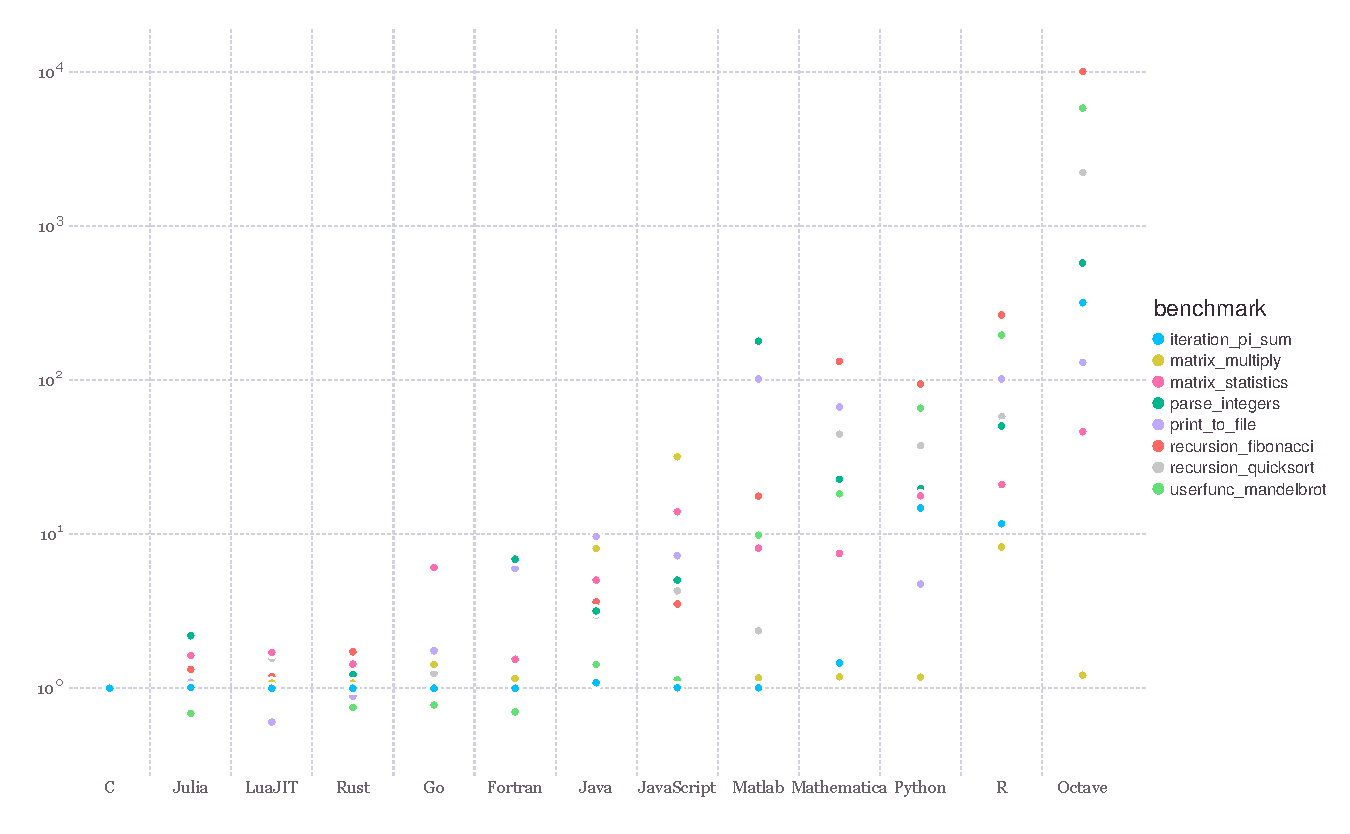
\includegraphics[width=\textwidth]{Figures/Chapter2/julia_benchmarks.pdf}
	\caption{Normalized benchmark time of some problems against the C implementation for different programming languages \cite{julia-benchmark}}
	\label{fig:julia_bench}
\end{figure}

In the context of this thesis, it can be expected that the code developed will be computationally intensive, given the fact that numerical integrators used to perform the propagation of the asteroids for the fitting procedure (which will undoubtedly run several times until a solution is identified), leading to a need for performance. In addition, coordinate transformations, missing objects from the images generated and other pitfalls require a productive way to deal with these problems. Since the two language problem is being faced, the decision has been made early to use Julia as the programming language for the development of this thesis.

\section{Orbital Dynamics}

For the description of the orbit determination problem being faced from the perspective of astrodynamics, we can simplify the problem into two separate problems, namely:

\begin{enumerate}
	\item The orbit followed by the Hera spacecraft during the observation period.
	\item The behavior of the two asteroids Didymos \& Dimorphos.
\end{enumerate}

Once an adequate description for both of these sub-problems has been given, they can then combine them into a single dynamics model using the appropriate reference frames and transformations between them. After this combination is complete, the image generation procedure can be built and different types of errors can be added.  
   
   
\subsection{Hera Spacecraft}

As briefly discussed in %insert chapter reference from Chapter 1
, the Hera spacecraft will follow hyperbolic trajectories. This is based on the legacy from a previous mission to a small body. The Rosetta mission visited the comet 67P/Churyumov-Gerasimenko in 2014. The Rosetta spacecraft implemented hyperbolic trajectories for a variety of reasons described by \citeauthor{rosetta-orbit} \cite{rosetta-orbit}, which include:

\begin{enumerate}
	\item Poor gravity potential estimates to plan an accurate circular or elliptic orbit.
	\item Large approach velocities for circular orbits when compared to orbital velocities.
	\item Lower sensitivity to insertion maneuver errors for hyperbolic trajectories. 
	\item The hyperbolic trajectory arcs can be designed in a manner which ensures that the sun remains behind the spacecraft at all times, providing good observation conditions. 
	\item The cost in terms of $\Delta v$ for the maintenance of the hyperbolic arcs remains fairly small, usually at the order of $\frac{\si{\centi\meter}}{\si{\second}}$.
\end{enumerate}

These problems remain applicable to the Didymos-Dimorphos asteroid system. Based on the expertise from Rosetta, ESA will command Hera to fly trajectories with pericentre velocity larger than the escape velocity, with a safety margin $C$, as defined in \Cref{eq:hera_velocity} \cite{hera-autonomous-ops}.

\begin{equation}
	\label{eq:hera_velocity}
	v_{p e r i}=(1+C) \sqrt{\frac{2 \mu}{r_{p e r i}}} \quad, \quad C>0
\end{equation}

The safety margin ensures that no collision can occur during an arc due to the presence of uncertainties in the gravity field model and is assigned a value of $C=0.4$ for Hera proximity operations \cite{hera-autonomous-ops}.

\subsection{SPICE and SPICE.jl}

Given all of this information, hyperbolic arcs can be defined at will. However, to ensure consistency with the actual implementation of Hera's orbit, the hyperbolic arcs of Hera will be extracted from SPICE. SPICE provides a portable, multi-discipline mechanism useful in both planning space science observations and defining the position of objects with respect to pre-defined reference frames \cite{SPICE}. SPICE is comprised of different logical elements which also form the acronym SPICE (Spacecraft, Planet, Instrument, Camera matrix and Events) and correspond to different SPICE data products which can then be used by end users for different applications\cite{SPICE}. An overview of the SPICE architecture can be found in \Cref{fig:spice_components}. Most notably, we are interested in the following SPICE kernels:

\begin{itemize}
	\item \textbf{SPK}, which provide position and velocity of spacecraft and different bodies as a function of time.
	\item \textbf{LSK}, which house the leapseconds kernel required for time computations. 
	\item \textbf{IK}, which house information about specific instruments on-board a spacecraft
	\item \textbf{CK}, which provide orientation of a camera instrument ("camera matrix") for specific time intervals.
	\item \textbf{FK}, which offer access to a number of reference frames which can then be used to transform coordinates between reference frames.
\end{itemize}

\begin{figure}[h]
	\centering
	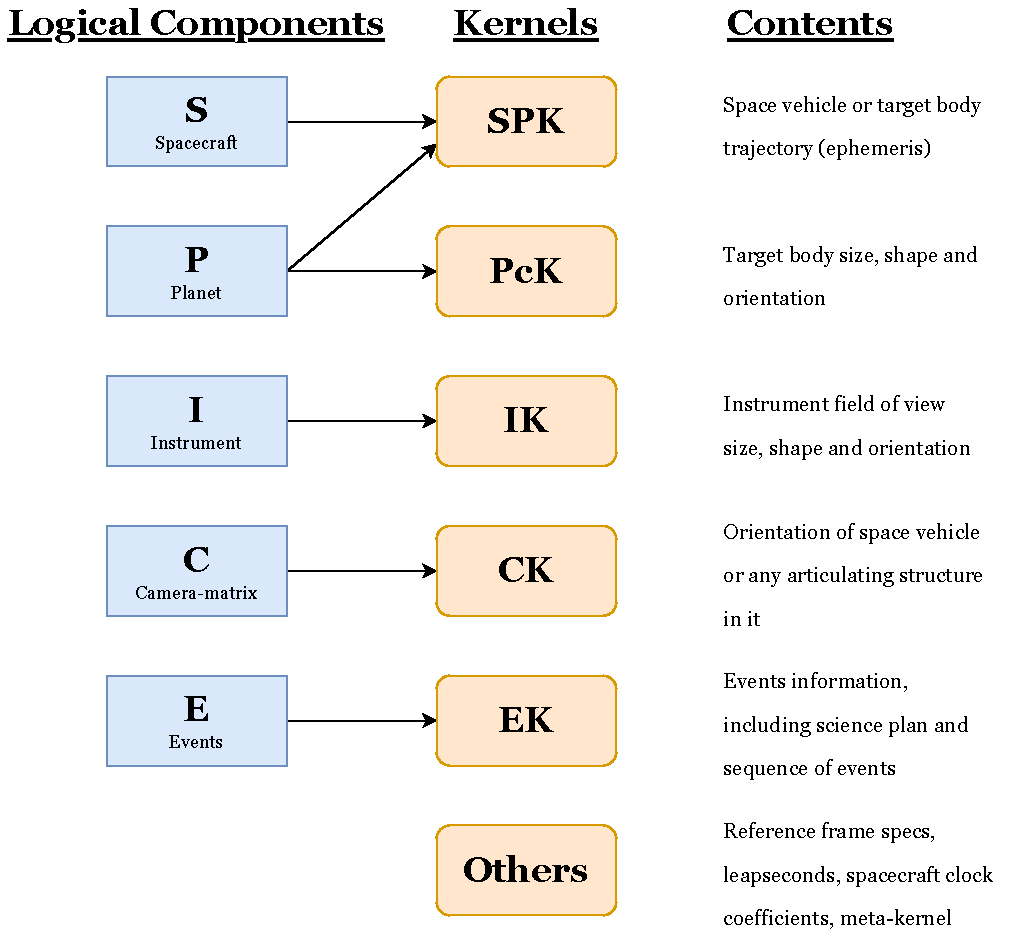
\includegraphics[width=\textwidth]{Figures/Chapter2/spice_components.pdf}
	\caption{Explanation of the SPICE architecture \cite{SPICE}}
	\label{fig:spice_components}
\end{figure}

The European Space Agency has a dedicated department called the ESA SPICE Service, which is located at the European Space Astronomy Center. ESA SPICE Service is responsible for the creation and distribution of SPICE data for a number of ESA missions, including the hera mission which is of interest to us \cite{esa-spice-hera}. The repository is updated every few months with the most up-to-date SPICE data based on revised estimates and/or new observational data. For this thesis, the Hera SPICE Kernel Dataset version 1.1 dated 09/11/2021 is used. To access the SPICE data provided, a dedicated Julia wrapper for the SPICE toolkit has to be used to convert the data to a usable format. This wrapper is SPICE.jl.  

As previously discussed in \Cref{chap:introduction}, the dynamical characterization of the Didymos-Dimorphos binary asteroid system takes place during the first of the six proximity operation phases, namely during the Early Characterization Phase \cite{hera-autonomous-ops}. During this phase, Hera performs hyperbolic arcs with the main objective of capturing images to perform a physical and dynamical characterization of the system \cite{hera-autonomous-ops}. Typical orbits followed by Hera during this phase can be seen in \Cref{fig:hera_extended_orbit}, which has been extracted directly from the SPICE data discussed before. In 

\begin{figure}[h]
	\centering
	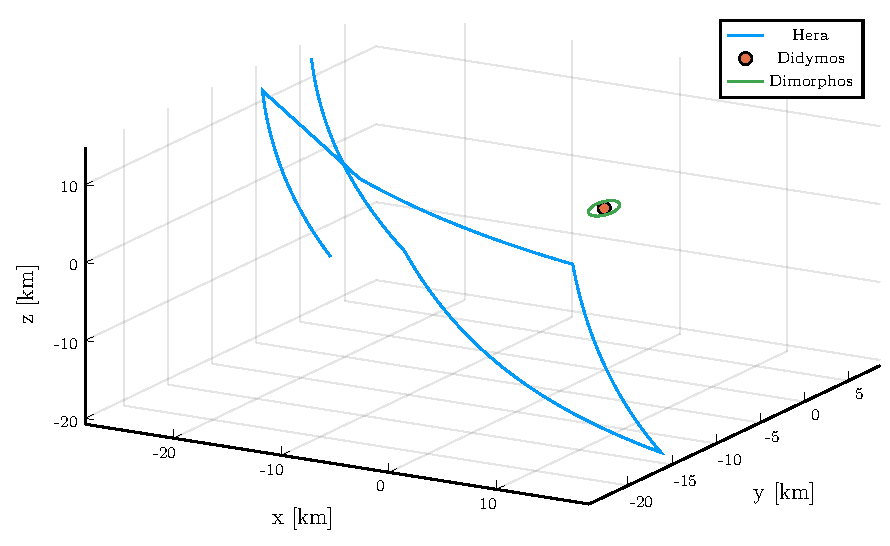
\includegraphics[width=\textwidth]{Figures/Chapter2/ECP_extended_reference_plot.pdf}
	\caption{Five hyperbolic arcs performed by Hera with respect to the system's barycenter over a period of 15 days.}
	\label{fig:hera_extended_orbit}
\end{figure}

For the context of this thesis, a narrower time interval has been chosen. The observation time used has been set to \si{120 \hour}, which is approximately equivalent to 10 orbits of Dimorphos around Didymos. This observation period is equal to \num{5} days, providing a reasonable time frame for the acquisition of pictures. At the worst case scenario, assuming that Hera has to acquire \num{500} photos of the two asteroids, approximately \num{4} photos per hour have to be taken, providing enough time per hour for other operations including orbital maintenance. The corresponding orbit of Hera for the selected time interval during the Early Characterization Phase with respect to the system's barycenter can be seen in \Cref{fig:hera_thesis_orbit}


\begin{figure}[h]
	\centering
	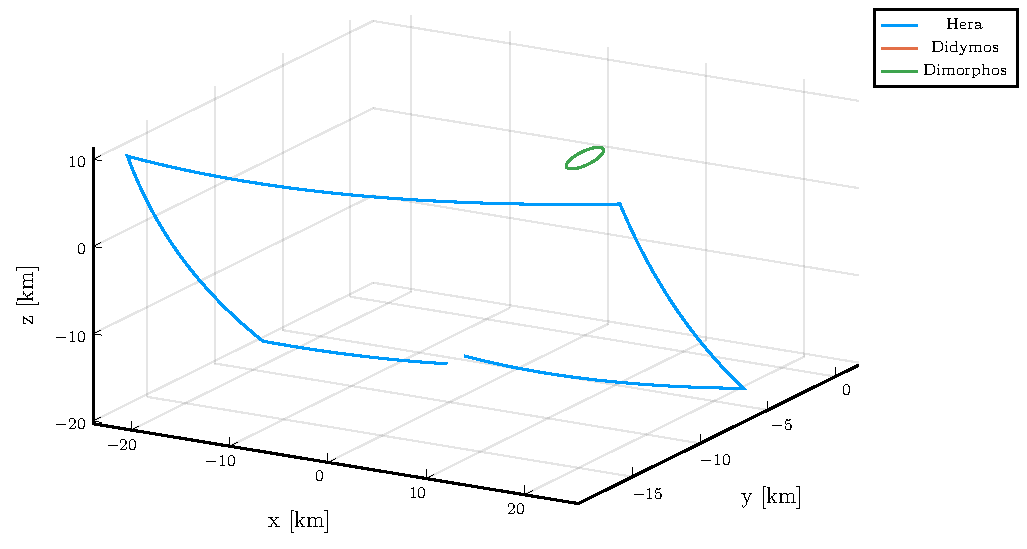
\includegraphics[width=\textwidth]{Figures/Chapter2/ECP_thesis_orbit_plot.pdf}
	\caption{The hyperbolic arcs which Hera orbits on during the \si{120\hour} observation period chosen for this thesis.}
	\label{fig:hera_thesis_orbit}
\end{figure}